\documentclass[conference]{IEEEtran}
\IEEEoverridecommandlockouts
% The preceding line is only needed to identify funding in the first footnote. If that is unneeded, please comment it out.
\usepackage{arydshln}
\usepackage{float}
\usepackage{booktabs}
\usepackage{array}
\usepackage{wrapfig} 
\usepackage{changepage}
\usepackage{listings}

\usepackage{multirow}
\usepackage{cite}
\usepackage{amsmath,amssymb,amsfonts}
\usepackage{algorithmic}
\usepackage{graphicx}
\usepackage{textcomp}
\usepackage[table]{xcolor}
\usepackage[unicode, pdftex]{hyperref}

\lstset{
	basicstyle=\small\ttfamily,
	language=Python,
	numbers=left,
	numberstyle=\tiny,
	numbersep=5pt,
	backgroundcolor=\color{gray!10},
	frame=single,
	breaklines=true,
	showstringspaces=false,
	tabsize = 2,
}
\def\BibTeX{{\rm B\kern-.05em{\sc i\kern-.025em b}\kern-.08em
    T\kern-.1667em\lower.7ex\hbox{E}\kern-.125emX}}

\newcommand{\reffig}[1]{Fig. \ref{#1}}
\newcommand{\refsec}[1]{Section \ref{#1}}
% \newcommand{\refeq}[1]{Eq. \ref{#1}}
\newcommand{\reftab}[1]{Table \ref{#1}}


\begin{document}

\title{Deployment of Frequency Regularization on Android Mobile Devices\
}

\author{\IEEEauthorblockN{1\textsuperscript{st} Wenhao You}
	\IEEEauthorblockA{\textit{Department of Computing Science} \\
		\textit{University of Alberta}\\
		Edmonton, Canada \\
		wyou1@ualberta.ca}
	\and
	\IEEEauthorblockN{2\textsuperscript{nd} Leo Chang}
	\IEEEauthorblockA{\textit{Department of Computing Science} \\
		\textit{University of Alberta}\\
		Edmonton, Canada \\
		basu@ualberta.ca}
}

\maketitle

\begin{abstract}
	
xxxxxxxxxxxxxxxxxxxxxxxxxxxxxxxxxxx

xxxxxxxxxxxxxxxxxxxxxxxxxxxxxxxxxxx

xxxxxxxxxxxxxxxxxxxxxxxxxxxxxxxxxxx

xxxxxxxxxxxxxxxxxxxxxxxxxxxxxxxxxxx

xxxxxxxxxxxxxxxxxxxxxxxxxxxxxxxxxxx

\end{abstract}

\begin{IEEEkeywords}
	
convolutional neural networks, frequency regularization.

\end{IEEEkeywords}

\section{Introduction}

Currently, people can not live without mobile devices. These compact yet powerful gadgets have become indispensable tools for communication, entertainment, and information. Their portability and versatility make them a constant companion. Meanwhile, Convolutional neural networks play an important role in computer vision applications. However, these neural networks are usually implemented on high-specification hardware. There are several advantages of running convolutional neural networks on mobile devices: privacy, internet, and runtime. For enhancing privacy, personal information does not need to be uploaded or transmitted to the cloud servers anymore. For reading the dependence on the internet connection, the functionality on local devices can replace some internet services. For the runtime, especially some applications that need real-time feedback, without connecting to the cloud server can shorten the processing time. In all, convolutional neural networks can totally replace the usage of many applications on mobile devices, ensuring personal data security. 

According to the popularity of mobile devices and the benefits of convolutional neural networks, we want to find a way to deploy some large and complex convolutional neural networks on mobile devices, leading to the question: “How can we deploy large convolutional neural networks on mobile devices?”

We found five methods to achieve our goal: upgrade the hardware of mobile devices; use Extreme Learning Machine (ELM)~\cite{anton2021elm} to allocate the weight of the hidden layers randomly in order to train large models on mobile devices faster; use NestDNN~\cite{fang2018nestdnn} dynamically adjust the size and computational complexity of the network based on available resources on mobile devices; use “One-shot Whole Network Compression”~\cite{kim2016oneshot} to prune, quantize, and compress the neural networks; use Frequency Regularization (FR)~\cite{zhao2023fr} to reduce parameters by removing high-frequency component. We make a more detailed introduction to their drawbacks and limitations in Section~\ref{related_work}.

After conducting a thorough literature review, considering all the limitations, accuracy, complexity, and future potential, we choose Frequency Regularization (FR) as our target algorithm, deploying it on one of the most popular mobile devices - Android mobile. Our main idea uses FR to compress a convolutional neural network U-Net and then decompresses the uploaded compressed model on an Android mobile device in a short time. After that, use the decompressed model to do image segmentation for the Carvana Image Masking Challenge Dataset~\cite{brian2017carvanadataset}. 

The proposed main idea can be divided into three directions to achieve the final goal respectively:
\begin{itemize}
	\item Direct deployment and tuning of FR code~\cite{fr_repo} on Android: Instead of introducing an additional operating system layer, this method focuses on deploying the Frequency Regularization (FR) algorithm within the Android ecosystem directedly. The core idea of this direction is to optimize and adjust the FR parameters specifically for the Android hardware and software architecture. 
	\item Deployment of Linux environment on Android system: It aims to add another layer to the Android system, providing a more controlled and flexible development environment for deploying and testing deep learning models. We choose Termux~\cite{termux_repo},~\cite{termux_overview},~\cite{termux_wiki} which is an Android terminal application and Linux environment to deploy. 
	\item Deployment of FR code on Android Studio: This method aims to optimize the FR algorithm for Android's native architecture, ensuring seamless integration and operation within Android. The main idea of this method is similar to the first direction above.
\end{itemize}	 		

\section{Related Work}\label{related_work}

Extreme learning machine (ELM) has been widely used in artificial intelligence field over the last decades~\cite{anton2021elm},~\cite{ding2014elmapp},~\cite{wang2022elmapp},~\cite{deng2015elmapp},~\cite{huang2006elmapp}. Although this algorithm has seen significant development, it also has several drawbacks: 
\begin{itemize}
	\item Poor tunability: It has poor controllability of the model since ELM calculates the least squares solution directly, and users cannot analyze the characteristics of the datasets to fine-tune. Adjusting models based on specific performance of mobile devices is important to mobile development.
	\item Lack of robustness: The performance of the model can be affected significantly while including certain outliers in different datasets, indicating poor robustness. Deployment on mobile devices needs to handle various inputs, including every potential outlier. Although there are many advanced versions of ELM~\cite{john2015advancedelm},~\cite{zhang2015advancedelm},~\cite{zhu2005advancedelm},~\cite{sun2017advancedelm} they lacks universality and are not as easy as other algorithms to deploy.
	\item Overfitting issues: While deploying large convolutional neural networks on mobile devices, model generalization is crucial since overfitting can result in poor performance on unseen data. ELM easily leads to overfitting issues because it is based on empirical risk minimization without considering structural risk. Xue et al.~\cite{ying2019overfit}pointed to a regularization strategy to solve this problem by feature-selection.
\end{itemize}	 

NestDNN is a framework that takes the dynamics of runtime resources into account~\cite{fang2018nestdnn}. The experiment of Fang et al.~\cite{fang2018nestdnn} achieves as much as 4.2\% increase in inference accuracy, 2.0× increase in video frame processing rate and 1.7× reduction in energy consumption. However, NestDNN also comes with some limitations. Its computational cost is significantly higher by using filter pruning method Triplet Response Residual (TRR). The high computational cost could probably exceed the processing capabilities of existing mobile devices and the runtime of model generation may be too long, which is not suitable for our deployment. 

``One-shot Whole Network Compression"~\cite{kim2016oneshot} includes removing certain parameters or structures, which is irreversible. Moreover, by using this compression method, the accuracy is too low. For example, in the experiment of Kim et al., by using AlexNet, the accuracy of the compressed model can drop by more than 50\%. In order to increase its accuracy, we have to make fine-tuning on the compressed model. Increasing accuracy requires at least more than 10 training epochs, which wastes too much time.

The proposed frequency regularization (FR)~\cite{zhao2023fr} works by restricting the non-zero elements of network parameters in the frequency domain, thus reducing information redundancy. Table~\ref{table:fr_unet} illustrates the evaluation of the proposed frequency regularization on UNet, according to compression rate, number of parameters, and dice score. Dice score is a metric for assessing the quality of image segmentation and ranges from 0 to 1, where 0 indicates no overlap and 1 indicates perfect overlap. The data under the dashed line represents the result under the most extreme condition in which only 759 float16 parameters are kept in UNet-v4. Thus, according to the surprised and satisfying experiment outcomes, we choose the frequency regularization as our compression method, to deploy it on mobile devices (i.e. Android system).

\begin{table}[H]
	\caption{Evaluation of the proposed frequency regularization on UNet for image segmentation tasks using Carvana Image Masking Challenge Dataset~\cite{zhao2023fr},~\cite{brian2017carvanadataset}.} 
	\label{table:fr_unet}
	\small
	\centering
	\begin{tabular}{p{1.15cm}rrr}
		\toprule
		&Dice Score&Compression Rate&\# of Parameters\\ 
		\midrule\midrule
		UNet-ref&99.13\%&100\%(1×)&31,043,586\\
		UNet-v1&99.51\%&1\%(100×)&310,964\\
		UNet-v2&99.37\%&0.1\%(1000×)&31,096\\
		UNet-v3&98.86\%&0.0094\%(10573×)&2,936\\
		\cdashline{1-4}
		UNet-v4&97.19\%&0.0012\%(81801×)&759(float16)\\
		\bottomrule
	\end{tabular}
\end{table}

Termux~\cite{termux_repo},~\cite{termux_overview},~\cite{termux_wiki}  is an Android terminal application and Linux environment. It works directly with no rooting or setup required. To use Termux, the system needs to meet some requirements: Android 5.0 - 12.0; CPU: AArch64, ARM, i686, x86\_64; at least 300 MB of disk space. It is open source and can be accessed at https://github.com/termux/termux-app. The instruction of deploy Termux on Android devices is available at https://github.com/btxcy/NeuralOnMobile\#readme. 

\section{Methodology}\label{methodology}
\subsection{Deployment on Android Devices}~\label{deployment}
To deploy the Frequency Regularization Compression Algorithm on Android devices, we have methodologies: using Termux to implement Linux environment on Android system and developing an Android Application with FR image segmentation by using Android Studio. 
\begin{itemize}
	\item\textbf{Termux:} "why we need termux, use for doing what"
	\item\textbf{Android Studio:} The reason for applying the algorithm by the Android Studio is because there is less memory consumption during the run. The logic of running on Termux is to create a virtual environment and run an operating system, in our experiment, Ubuntu. Although we are running the compact version of Ubuntu, the limitation is that Ubuntu does not recognize the type of device we are running on. Therefore, it brings up the problem of installing the incapable PyTorch or other libraries. Whereas on an Android application, there is no virtual environment involved. 
	\begin{itemize}
		\item Normal FR on Android Application:
		\item 4-parts FR on Android Application:
	\end{itemize}	 		
\end{itemize}	 		

\subsection{Qualitative and Quantitative Metrics}~\label{metrics}
To analyze the results of our experiment, we have three qualitative and quantitative metrices: usage of random access memory, dice score, and visual perception.
\begin{itemize}
	\item\textbf{Usage of Random Access Memory (RAM): }
	% As we run the algorithm on mobile devices, the compressing algorithm Frequency Regularization becomes more significant in this experiment. Mobile device manufacturers increase their memory storage and CPUs to highlight their performance. There are some methods we implemented during the research to compress memory usage. For instance, when running the U-Net neural network layers, saving the outputs in the local storage helps to decrease memory usage. The reason is that output tensors from each layer contain large sizes to store in the memory. But by saving them locally, we can instantly free the memory without occupying it. The next layer can easily access the tensors from the local storage instead of the memory. It helps to reduce about two gigabytes of random memory usage. There is another method to reduce memory usage. As the algorithm requires more memory than the original neural network model from PyTorch, we can make the Frequency Regularization algorithm run only once when initializing the neural network. However, the method does not have a dramatic decrease in memory usage as the previous method. 
	\item\textbf{Dice Score:}
	\item\textbf{Visual Perception:}
\end{itemize}	



\section{Experiments} 
\subsection{Packaging frequency regularization Project}~\label{package_fr}
As current and future plans of Zhao et al.~\cite{fr_repo},~\cite{zhao2023fr}, we have accomplished the development of a pip repository for their Frequency Regularization technique and committed to their original repository. We can now integrate Frequency Regularization into our project by simply running the command line in Linux environment:

	\begin{verbatim}
		$ pip install frereg
	\end{verbatim}

This step is instrumental in simplifying the deployment of condensed yet potent models in pragmatic applications. We will use this python library in Section~\ref{build_linux}.

\subsection{Build Linux environment and install the frequency regularization package} ~\label{build_linux}
We utilized an Android device which ran version 12.0.1 for this section. In order to facilitate the deployment of an Ubuntu environment within the Android system, we downloaded Termux~\cite{termux_repo},~\cite{termux_overview},~\cite{termux_wiki} , which version is v0.118.0. Upon accessing Termux, we employed a suite of basic tools, such as wget, proot, and git, to establish the Ubuntu environment. The Ubuntu package~\cite{ubuntu_in_termux_repo} we used is quite different from the conventional Ubuntu installations on normal personal computers. For more detailed steps of setting up the environment, please check our source code repository~\cite{nerual_on_mobile_repo}. After initiating the Ubuntu environment and installing both Python and the Python-pip tool, we used the command line we mentioned in Section~\ref{package_fr}, installing the frequency regularization project successfully.


\subsection{Deployment of Android Studio}
As mentioned in Section~\ref{deployment}, the system can install an incapable PyTorch function through the virtual environment with mobile devices. Therefore, running the Python Script on the Android Studio required the python library Chaquopy~\cite{chaquopy2023} in this research. It helps us to implement the \textit{pip} library from Python. However, in some situations, some PyTorch features may still not work when running the code because of the difference in hardware structure between the computer and mobile devices~\cite{fojtik2022cpu}. For instance, the Discrete Fast Fourier Transforms, mobile devices do not support this operation due to the requirement of GPU involvement. Therefore, an alternative solution is to convert the tensor data to the NumPy array, which runs through the CPU. After the transformation, we then convert back to the PyTorch tensor array. Many functions require conversion to make it work in the Frequency Regularization algorithm. 

We show the outputs from the algorithm running on an Android phone by making an application using Android Studio to run the Frequency Regularization. The only feature the application provides currently is importing the images from the local machine directory. After that, we get the output from the compressed neural network. 

The left-hand column of the ~\ref{image:3_outputs} shows the original images we want to implement the image segmentation. From left to right, the three columns represent three outputs generated by an Android phone respectively: output from non-compressed model, output from FR compressed model, output from FR compressed model with 4 parts. Table~\ref{table:ram_usage} illustrates the results among three ways of image segmentation. \textbf{{analyze the avg. values here!}}

% The middle images are the desired images of the segmented results. The right-hand side is the result of the implementation. The results are worse than the desired segmented images since we are trying to compress the memory usage. The implementation idea is to cut the original images into four pieces. After the process, we take the cut results into the neural network. Finally, we concatenate each result into one to restore its original state. The method compressed memory usage a lot \textbf{(need table here)}. However, the result of the dice score is not what we expected as the computer's.  


\begin{table}[H]
	\caption{Comparison of RAM Usage for Image Segmentation for Carvana Image Masking Challenge Dataset~\cite{brian2017carvanadataset} on an Android Phone: Uncompressed U-Net, FR Compressed and Decompressed U-Net, and FR Compressed and Decompressed U-Net Processing Four Parts of an Image Simultaneously.} 
	\label{table:ram_usage}
	\small
	\centering
	\begin{tabular}{rrrr}
		\toprule
		&Non-compressed&Compressed&Compressed(4-parts)\\
		\midrule\midrule
		1$^{st}$ Avg.&4.2966GB&1.2324GB&1.2553GB\\
		2$^{nd}$ Avg.&4.2966GB&1.2858GB&1.1073GB\\
		3$^{rd}$ Avg.&4.2966GB&xxxxx&1.2546GB\\
		\cdashline{1-4}
		Total Avg.&4.2966GB&xx&1.2057GB\\
		\bottomrule
	\end{tabular}
\end{table}

\begin{table}[H]
	\caption{Dice Scores} 
	\label{xxx}
	\small
	\centering
	\begin{tabular}{rrrr}
		\toprule
		&Non-compressed&Compressed&Compressed(4-parts)\\
		\midrule\midrule
		1$^{st}$ Avg.&0.9718&0.9716&0.7567\\
		2$^{nd}$ Avg.&xx&0.9718&0.7567\\
		3$^{rd}$ Avg.&xx&xx&0.7567\\
		\cdashline{1-4}
		Total Avg.&xx&xx&0.7567\\
		\bottomrule
	\end{tabular}
\end{table}
% the image needs to be redo
% separate original image with the results
% result image: LHS: result of the computer, RHS: result of the phone implementation
\begin{figure}[htbp]
	\centering
	\label{image:3_outputs}
	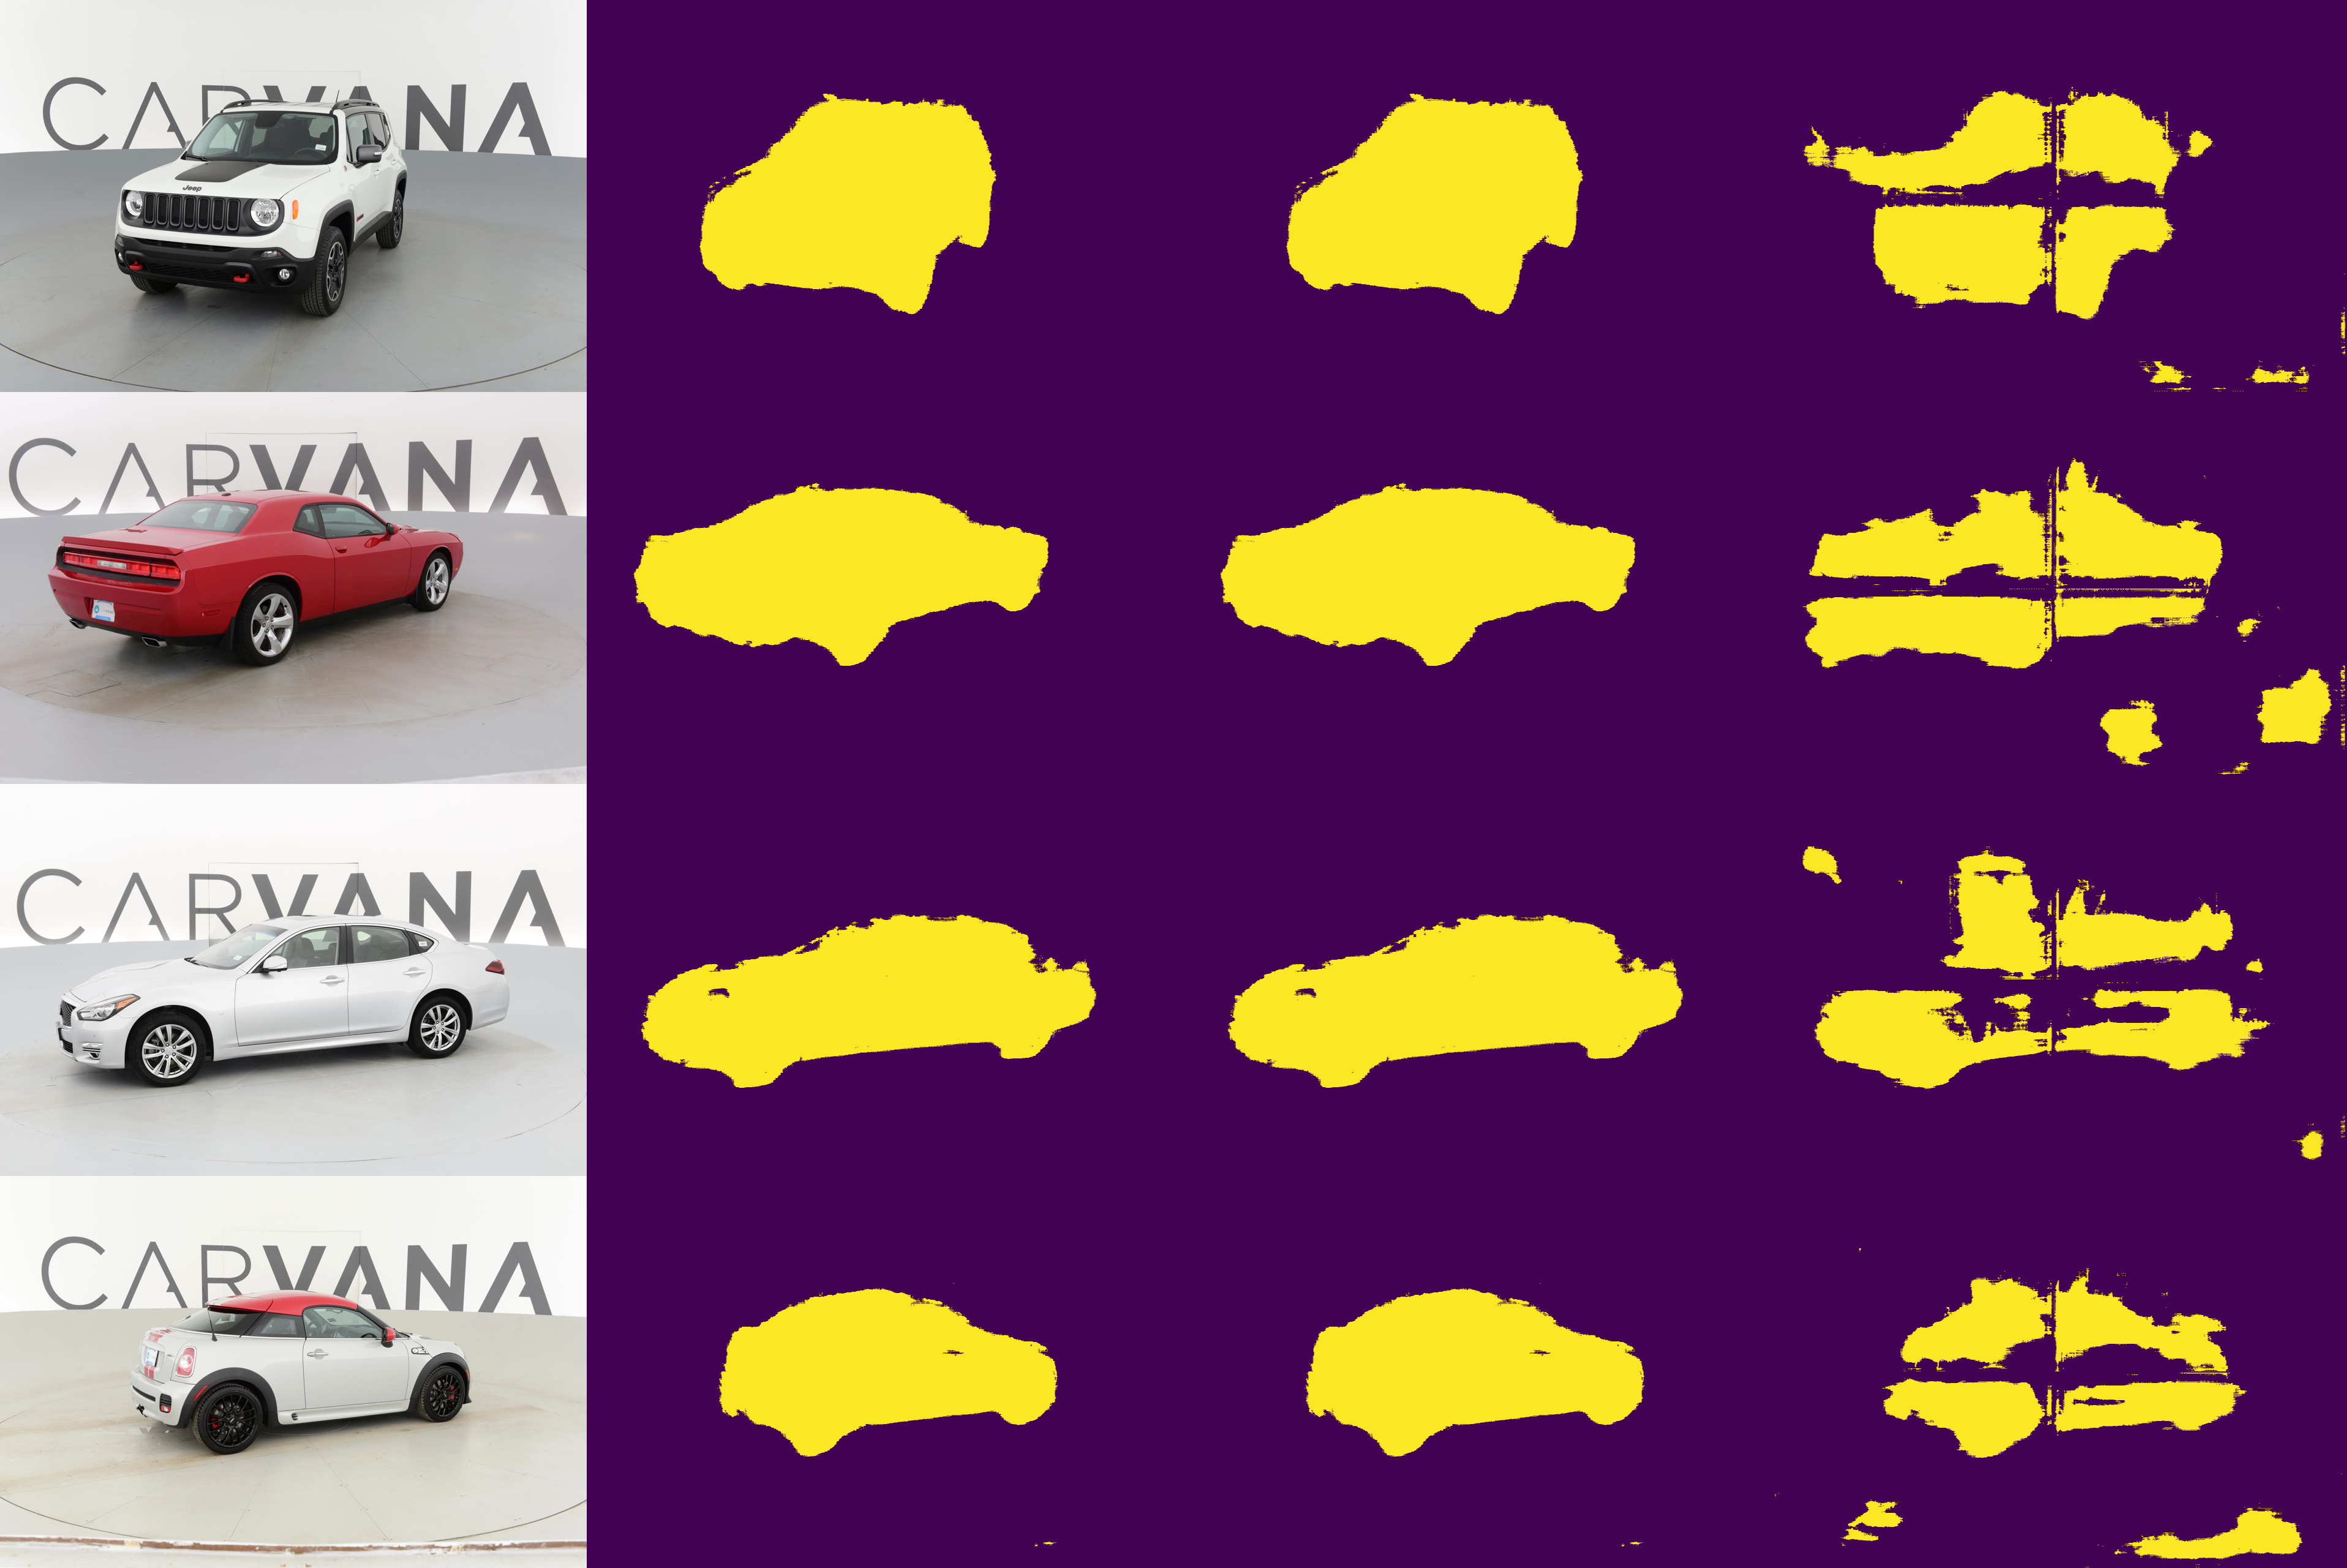
\includegraphics[width=1\linewidth]{figures/3_outputs.png}
	\caption{Comparison between Original Images and Outputs from Image Segmentation for Carvana Image Masking Challenge Dataset~\cite{brian2017carvanadataset} on an Android Phone: Uncompressed U-Net, FR Compressed and Decompressed U-Net, and FR Compressed and Decompressed U-Net Processing Four Parts of an Image Simultaneously.}
\end{figure}



\section{Limitation and Future Work} 
xxxx

\section{Conclusion} 
xxxx

\bibliographystyle{IEEEtran}  
\bibliography{ref}

\end{document}
